%%%%%%%%%%%%%%%%%%%%%%% file typeinst.tex %%%%%%%%%%%%%%%%%%%%%%%%%
%
% This is the LaTeX source for the instructions to authors using
% the LaTeX document class 'llncs.cls' for contributions to
% the Lecture Notes in Computer Sciences series.
% http://www.springer.com/lncs       Springer Heidelberg 2006/05/04
%
% It may be used as a template for your own input - copy it
% to a new file with a new name and use it as the basis
% for your article.
%
% NB: the document class 'llncs' has its own and detailed documentation, see
% ftp://ftp.springer.de/data/pubftp/pub/tex/latex/llncs/latex2e/llncsdoc.pdf
%
%%%%%%%%%%%%%%%%%%%%%%%%%%%%%%%%%%%%%%%%%%%%%%%%%%%%%%%%%%%%%%%%%%%

\documentclass[runningheads,a4paper,10pt]{llncs}

\usepackage[utf8]{inputenc}
\usepackage[left=3cm,right=3cm,top=3cm,bottom=3cm]{geometry}

\usepackage{natbib}
\bibliographystyle{apalike-fr}

\usepackage{amssymb}
\setcounter{tocdepth}{3}
\usepackage{graphicx}

\usepackage[hidelinks]{hyperref}
\usepackage[title]{appendix}

\usepackage{caption}

\usepackage{amsmath}

\usepackage{fourier-orns}

\usepackage[french]{babel} % Pour adopter les règles de typographie française
\usepackage[T1]{fontenc} % Pour que les lettres accentuées soient reconnues

%ALGORITHM
\usepackage{algorithm}
\usepackage[noend]{algpseudocode}
\renewcommand{\algorithmicforall}{\textbf{for each}}
\newcommand{\var}[1]{\mathit{#1}}
\newcommand{\func}[1]{\mathrm{#1}}
\algdef{SE}[DOWHILE]{Do}{doWhile}{\algorithmicdo}[1]{\algorithmicwhile\ #1}
%

\usepackage{url}
\urldef{\mailsa}\path|{alfred.hofmann, ursula.barth, ingrid.haas, frank.holzwarth,|
\urldef{\mailsb}\path|anna.kramer, leonie.kunz, christine.reiss, nicole.sator,|
\urldef{\mailsc}\path|erika.siebert-cole, peter.strasser, lncs}@springer.com|    
\newcommand{\keywords}[1]{\par\addvspace\baselineskip
\noindent\keywordname\enspace\ignorespaces#1}

\begin{document}

\mainmatter 

\title{Mini Mémoire \\ Le Model-Checking de CTL}

\titlerunning{Le Model-Checking de CTL}

\author{BUI QUANG PHUONG Linh -- 000427796 \\ Promoteur : Prof. GEERAERTS Gilles \\ Année 2017-2018}

\institute{Université Libre de Bruxelles}

\authorrunning{BUI QUANG PHUONG Linh}

\toctitle{Abstract}
\tocauthor{{}}

\maketitle


\begin{abstract}
La vérification de modèles, plus communément appelée via son appellation anglaise \textit{Model-Checking}, est un système de vérification automatique qu'un système informatique ou électronique satisfasse une certaine propriété. Celle-ci est généralement utilisé afin de prouver la bonne fonctionnalité du système ou dans le cas contraire, de détecter des bugs ou des dysfonctionnements. Plusieurs types d'algorithmes et de logiques permettent d'effectuer un Model-Checking. Nous allons principalement nous intéresser au Model-Checking de CTL mis en place durant les années 80. 
\end{abstract}

\medskip

\begingroup
\let\clearpage\relax
\tableofcontents
\endgroup

\medskip
\medskip

\newpage 

\section{Introduction}

\subsection{Contexte et point de vue global}
\noindent
Les dernières décennies entrainant l'évolution exponentielle de la technologie et de l'informatique, la société actuelle fait régulièrement usage de systèmes automatisés afin d'assurer le bon fonctionnement et la fiabilité des programmes, machines et autres divers systèmes informatiques. Afin de vérifier ces systèmes, l'utilisation d'une technique algorithmique appelée \textit{Model-Checking} va être mise en place.  

\noindent
Le principe de base du model-checking est la vérification qu'un certain système satisfasse une certaine propriété. Le système sera représenté par un modèle $\mathcal{M}$ tandis que la propriété fera office d'une formule $\Phi$. Dans un premier temps, la modélisation du comportement dynamique du système est nécessaire avant d'être suivie par la vérification de la formule de la propriété grâce à l'algorithme de model-checking qui déterminera si le modèle satisfait bien la formule.  

$$\boxed{\mathcal{M} \vDash \Phi}$$

\noindent
Lorsque le système ne satisfait pas la propriété évaluée, le model-checking a donc repéré un bug ou un dysfonctionnement. Chaque année, le coût des bugs s'élève à environ 59 milliards de dollars \cite{ErrorCost} rien qu'aux Etats-Unis. La création et la mise en place de technique de vérification est donc impérative pour réduire le taux de bugs afin de minimiser ces coûts.  \\

\noindent
Illustrons cela par un exemple plus concret : un distributeur de boissons. Dans ce cas, il est indispensable que le montant demandé pour une certaine boisson soit mis dans la machine afin que le client puisse récupérer la boisson. La vérification de ce prérequis va être effectuée à l'aide d'un système de model-checking. 
Un autre exemple illustrant l'importance du model-checking est la fermeture des barrières sur une voie ferrée lors du passage d'un train. 
Celle-ci doit être réalisée automatiquement lorsqu'un train est sur le point de traverser une voie ferrée. Dans ce cas, une petite erreur de timing peut avoir une très grande ampleur concernant la sécurité des passants. Il est donc impératif de vérifier la bonne fonctionnalité du système gérant la fermeture des barrières grâce au model-checking. 

\noindent 

\subsection{Les phases du model-checking}

Le processus de base d'un model-checking est divisé en 3 phases : 

\begin{enumerate}
 \item  \textbf{La phase de modélisation} : permet de représenter le comportement du système. Dans le cas du model-checking, cette phase de modélisation est réalisée à l'aide d'automates d'états finis\footnote{cfr. \autoref{sec:pdv-algo} "Algorithme de model checking"} et de logique temporelle\footnote{cfr. \autoref{sec:log-temp} "Introduction à la logique temporelle"}. Celle-ci permet une formalisation du système ainsi que de la propriété à vérifier. De plus, cette modélisation permet de réaliser les premières vérifications grâce à différentes simulations réalisées sur le modèle. Cette phase de modélisation est l'objet de la \autoref{sec:pdv-algo} \textit{"Algorithme de model checking"} et \autoref{sec:log-temp} \textit{"Introduction à la logique temporelle"}. 
 \item  \textbf{La phase d'exécution} : exécution du model-checker vérifiant la validité de la propriété à satisfaire. Le model checking trouve principalement son intérêt dans sa vérification \textbf{automatique} et offre donc un réel avantage. (cfr. \autoref{sec:avantages})   
 \item  \textbf{La phase d'analyse} : lorsque les résultats sont obtenus après exécution, différents cas potentiels existent : 
 \begin{itemize}
 \item Si la propriété est \textbf{satisfaite} : vérification de la propriété suivante (s'il y en a). 
 \item Si la propriété n'est \textbf{pas satisfaite} : soit un contre-exemple est produit qui décrit un scénario possible d’erreur (violation de la propriété), soit il y a correction du modèle et réexécution du model-checker, soit il y a réexécution de toute la procédure. 
 \item \textbf{Manque de mémoire} (cfr. \textit{State explosion problem}\footnote{\autoref{sec:desavantages} - 1er désavantage}): tentative de réduction du modèle notamment grâce aux diagrammes de décision binaire ou une réduction partielle de la commande et réexécution le model-checker. 
 \end{itemize}
 \end{enumerate} 
 
Un schéma récapitulatif reprenant les différentes phases citées ci-dessus est présentée dans la \autoref{fig:schematic-view}.
 
\begin{figure}
  \centering
   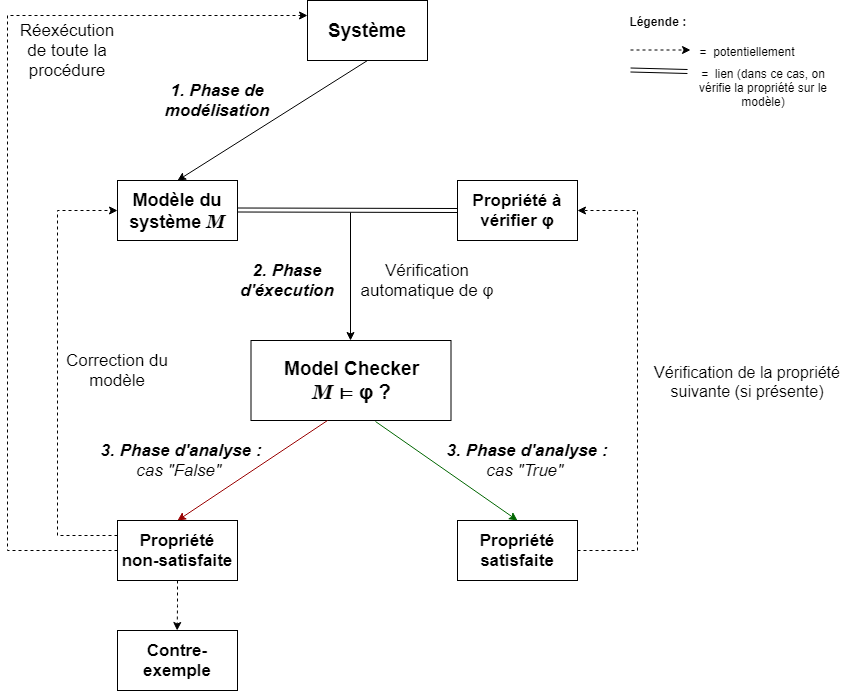
\includegraphics[scale=0.45]{figures/Diag_Recap_MC.png}
   \caption[Caption for LOF]{Schéma récapitulatif de l'approche du model-checking}
   \label{fig:schematic-view}
\end{figure}

\subsection{Avantages \& désavantages}

Dans cette section, plusieurs avantages et inconvénients seront présentés sur base des recherches effectuées en 2008 par \textit{Clarke} \cite{Birth-MC} ainsi que du livre de référence "Principles of Model Checking" \cite{RefBook}.

\subsubsection{Avantages du model-checking} \label{sec:avantages}

Le model-checking possède plusieurs avantages par rapport à l'utilisation d'éventuelles autres techniques de vérifications et de détection d'erreur. Voici une liste non exhaustive de ces avantages : 

\begin{itemize}
\item Il s'agit d'une approche générale de vérification applicable dans tous les domaines tels que les systèmes embarqués ou ingénierie logicielle. 
\item La phase de vérification est automatique. Suivant la phase de modélisation, la seule action nécessaire de l'utilisateur afin de faire fonctionner le model-checking est de l'activer. Le programme s'occupe du reste. Niveau performance, cet automatisme permet un gain de temps conséquent. 
\item Contrairement aux simples tests, le model-checking va également prouver la bonne fonctionnalité du système et dans le cas contraire, nous renvoyer un contre-exemple d'une exécution du système qui falsifie la propriété et ainsi, détecter le(s) bug(s). Le taux d'erreurs non repérées est donc moindre par rapport aux tests simples. 
\item Le model-checking agit sur toute la modélisation du système et non qu'une seule partie, il s'agit donc d'une méthode exhaustive. Néanmoins, si l'utilisateur le souhaite, il est tout de même possible d'utiliser le model-checking pour une vérification partielle et ainsi l'appliquer à des parties de la modélisation. 
\item Utilisation de la logique temporelle (\textit{cfr. \autoref{sec:log-temp} "Introduction à la logique temporelle"}) qui permet d'exprimer facilement les diverses propriétés de manière non ambigüe et universelle. 
\end{itemize}

\subsubsection{Désavantages du model-checking} \label{sec:desavantages}

Néanmoins, le model-checking est une solution discutable sur certains points : 

\begin{itemize}
\item Lorsqu'un problème est traité par la technique de model checking, plus un problème est grand, plus la taille du model checking va croître. Le modèle réalisé va donc grandir exponentiellement au nombre de processus actifs (appelés états). Pour $N$ variables avec un domaine de $k$ valeurs possibles, le nombre d'états grandit de $k^{N}$. Par exemple, pour 20 variables booléennes, il y aurait déjà $2^{20}$ soit 1048576 états. Le modèle devient donc très vite surchargé et surpasse la capacité de la mémoire. Ce problème est appelé \textit{State explosion problem} \cite{StateExpProb}. Par conséquent, le model-checking ne pourrait donc pas croître. Cependant, plusieurs recherches \footnote{La section 5 "State Explosion Problem" de l'article de Clarke \cite{StateExpProb} reprend les principales recherches de solutions à ce problème.} ont été établies dans le but d'établir une solution à ce problème tels que les \textit{diagrammes de décisions binaires} permettant de représenter plusieurs états en un diagramme. 
\item Le model-checking s'applique généralement sur des systèmes finis et n'est pas adapté aux systèmes non-finis de part sa modélisation grâce à des automates d'états finis. Hors, la possibilité de tomber sur un système non-fini (ayant donc une infinité de valeurs possibles pour les variables) n'est pas écartée. 
\item Comme son nom l'indique, le model-checking exécute une vérification du modèle du système et non du système en lui-même. Le modèle étant limité à un système de transitions (cfr \autoref{sec:pdv-algo} \textit{"Algorithme de model checking"}), ce n'est donc pas une représentation exacte du système, certains éléments pourraient différés et/ou manqués, que ce soit au niveau du hardware tel que des défauts de fabrication ou bien au niveau software tel que des erreurs de codage. Pour palier à ce problème, des tests supplémentaires sont nécessaires. 
\item Conséquence du dernier point : le résultat n'est donc pas garanti à 100\% et pourrait donc contenir des erreurs. 
\end{itemize}

\section{Algorithme de model checking} \label{sec:pdv-algo}

\subsection{Graphes et principes d'états}
%Présentation du principe de systèmes d'états finis et de graphes en quelques mots + Schéma 
Le model-checking base sa représentation sur un système de graphe orienté, plus précisément sur un \textit{système d'états finis} où chaque n\oe ud du graphe est appelé état tel que les arcs entre ces états sont appelés transitions. Cet ensemble d'états et de transitions décrit le comportement du système réactif et forme le \textbf{modèle} de ce système. Dans l'exemple du problème de distributeur de boissons abordé précédemment, un tel modèle se présenterait comme tel: 

\begin{figure}
  \centering
   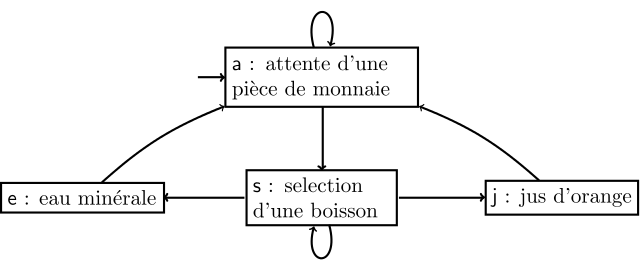
\includegraphics[scale=0.4]{figures/model-boissons.png}
   \caption[Caption for LOF]{Modèle du problème d'un distributeur de boissons \cite{wiki}}
   \label{fig:model_boissons_1}
\end{figure}

\noindent
où chaque état est défini par un nom (un alias). Par exemple, "a" définit l'attente de l'entrée d'une pièce de monnaie dans la machine. \\

Un modèle de ce type constitue la base d'une \textit{structure de Kripke}. La section suivante présente une telle structure ainsi que l'adaptation du modèle de la \autoref{fig:model_boissons_1} en \textit{modèle de Kripke}. 

\subsection{Structure de Kripke} \label{sec:kripke}
%Présentation de la structure de Kripke, définitions des différentes notions.

\subsubsection{Définition} 

Une structure de \textit{Kripke} \cite{Kripke} est un tuple : 

$$\boxed{\mathcal{K} = (S,I,A,AP,\longrightarrow,\lambda)}$$ 

\noindent
tel que : 
\begin{itemize}
\item \textbf{S} est un ensemble fini d'états, \\
\item \boldmath$I \subseteq S$ est l'ensemble des états initiaux, \\
\item \textbf{A} est un ensemble d'actions, \\
\item \textbf{AP} est un ensemble de propositions atomiques, \\
\item \boldmath$\longrightarrow \hspace{0.2cm} \subseteq S \times A \times S$ est une relation de transitions entre états, \\
\item \boldmath$\lambda : S \rightarrow 2^{AP}$ est une fonction de labelisation (étiquetage) des états qui définit pour chaque état $s \in S$ l'ensemble $\lambda(s)$ de toutes les propositions atomiques $AP$ qui sont valides dans cet état. 


\end{itemize}

\subsubsection{Exemple complet d'une structure de Kripke} 

Toujours sur base du même problème de distribiteur de boissons, le modèle de la \autoref{fig:model_boissons_1} peut-être repris et complété en se voyant attribuer des noms d'actions afin de pouvoir spécifier les transitions et par conséquent de respecter la structure de Kripke. 

\begin{figure}
  \centering
   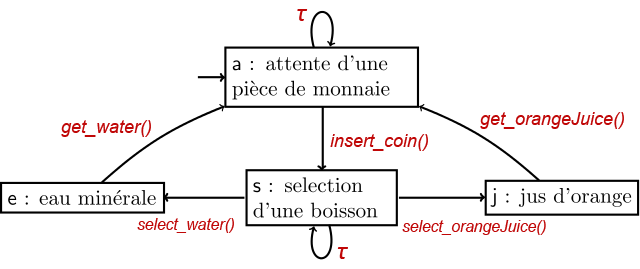
\includegraphics[scale=0.5]{figures/model-boissons-2.png}
   \caption[Caption for LOF]{Modèle de Kripke complet du problème d'un distributeur de boissons}
   \label{fig:model_boissons_2}
\end{figure}

\noindent
Dans ce cas, l'ensemble des états est $S = \{a, e, s, j\}$. L'ensemble des états initiaux $I = \{a\}$ ici ne comporte qu'un seul état initial et est représenté dans le modèle par un arc d'entrée vers l'état initial $a$. \\

\noindent
Les labels associés à chaque transition correspond à une action et font donc partie de l'ensemble d'action $A$. Le symbole $\tau$ représente une action silencieuse qui désigne une action non observable mais qui n'est néanmoins pas à négliger tels que l'attente de la pièce ou une non-sélection de boisson. \\
L'ensemble d'action est donc $A = \{select\_water, select\_orangeJuice, insert\_coin, get\_orangeJuice, \tau\}$. \\

\noindent
Les états et actions maintenant définis, des exemples de relations de transitions peuvent être présentés. Voici les transitions d'états lors de l'achat d'un jus d'orange dans le distributeur : 

\begin{enumerate}
\item \boldmath$a \xrightarrow{\text{insert\_coin()}} s$ : représente la transition de l'état \textit{attente d'une pièce de monnaie} à l'état \textit{sélection d'une boisson} grâce à l'action d'insertion de pièce \textit{insert\_coin}. 
\item \boldmath$s \xrightarrow{\text{select\_orangeJuice()}} j$ : représente la transition de l'état \textit{sélection d'une boisson} à l'état \textit{jus d'orange} grâce à l'action \textit{select\_orangeJuice}. 
\item \boldmath$j \xrightarrow{\text{get\_orangeJuice()}} a$ : représente la transition de l'état \textit{jus d'orange} à l'état \textit{attente d'une pièce de monnaie} grâce à l'action \textit{get\_orangeJuice}.
\end{enumerate} 

Ces 3 exemples de transitions font partie des 7 transitions d'états possibles du modèle. \\

\noindent
Finalement, concernant le choix des propositions atomiques, le choix le plus simple est d'utiliser le nom des états comme propositions atomiques.\\
Pour un état $s$, la fonction de labelisation serait donc $\lambda(s) = \{s\} \cap AP$.  

\subsection{Arbre d'exécution d'une structure de Kripke}

\subsubsection{Définition} 
Un \textit{arbre d'exécution d'une struture de Kripke} correspond au "dépliage" du modèle de Kripke où les n\oe uds correspondent aux états tel que la racine est l'état initial du modèle de Kripke. Au niveau $i$, les fils d'un n\oe ud sont les états successeurs au niveau $i+1$, c'est-à-dire les états subissant une transition à partir du n\oe ud du niveau $i$. 

\subsubsection{Pourquoi utiliser un arbre ?}
L'utilisation d'un arbre permet de représenter tous les chemins de la structure de Kripke. Lorsque le graphe de Kripke est cyclique, l'arbre résultant est un arbre infini. C'est notamment de cette transformation en arbre que \textbf{le model checking CTL} (Computation Tree Logic) tient son nom vu qu'il se base sur la structure en arbre du système. 

\subsubsection{Illustration : d'un graphe à un arbre.}

Afin d'illustrer la transformation de la structure de Kripke à un arbre, reprenons une nouvelle fois l'exemple du distributeur de boissons dont le modèle de Kripke est présentée à la \autoref{fig:model_boissons_2} et transformons celui-ci en arbre. 

\begin{figure}
  \centering
   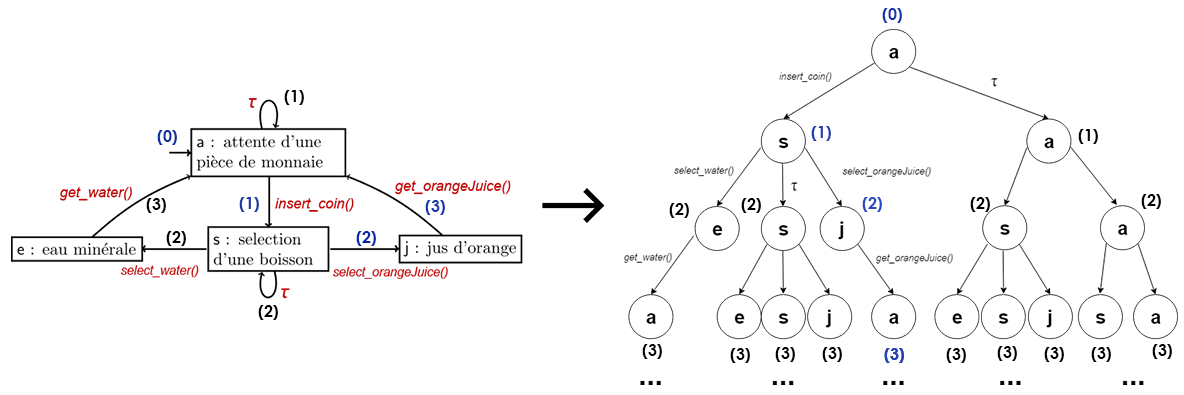
\includegraphics[scale=0.37]{figures/Arbre_Distributeur_V2.png}
   \caption[Caption for LOF]{Etapes de construction de l'arbre à partir du graphe}
   \label{fig:arbre_boissons}
\end{figure}

La \autoref{fig:arbre_boissons} présente les différentes étapes de construction de l'arbre d'exécution de la structure de Kripke du problème du distributeur de boissons vu précédemment. 
La construction débute par l'état initial du système et va donc représenter la racine de l'arbre (Niveau 0). Le niveau suivant (Niveau 1) représente les états successeurs potentiels de l'état précédent, à savoir l'état intial 0. Dans la même logique, le niveau 2 contient les états potentiels successeurs de ceux du niveau 1, et ainsi de suite pour tous les niveaux. En guise d'exemple d'exécution, l'achat d'un jus d'orange est représenté par les états dont leurs numéros sont bleus dans la \autoref{fig:arbre_boissons}. \\

Tous les éléments présents dans le modèle de Kripke se retrouvent bien dans l'arbre. Dans ce cas, il s'agit bien d'un arbre infini résultant d'un graphe cyclique dont les 4 premiers niveaux sont présentés dans la \autoref{fig:arbre_boissons}.

 
\section{Le model-checking de CTL: généralités et logiques}

\subsection{Introduction à la logique temporelle} \label{sec:log-temp}
%Première approche de la notion de logique temporelle, des différentes sortes de logiques temporelles existantes (linéaire ou arborescente), des propositions de logiques temporelles, des formules associés, ... 
Les différentes propriétés du système à vérifier sont exprimés via la notion de \textit{logique temporelle}. Celle-ci forme le deuxième élément complémentaire aux systèmes d'états finis (modèle de Kripke) permettant la réalisation de l'étape de modélisation du model checking. 

La logique temporelle définit les propriétés temporelles à l’aide de connecteurs temporels\footnote{N.B: Il s'agit bien d'une logique temporelle et non temporisée, cette logique ne quantifie donc pas l'écoulement du temps mais décrit bien l'ordre des événements sans introduire la notion de temps explicitement.} ("until", "next", "always", ...) et de quantificateurs sur les états ou les chemins de son graphe. Cette logique permet donc d'exprimer et vérifier des propriété de sûreté (absence de bugs), d’absence de blocages de l’exécution, d'invariance (tous les états satisfont une propriété) ou d'équité (fonctionnel et répétable infiniment) et remplit donc parfaitement le rôle de vérification du model checking. \\

Les deux principaux types de logiques temporelles qui seront abordés prochainement sont \textbf{la logique temporelle linéaire} (LTL) et \textbf{la logique temporelle arborescente} (CTL). Cependant, il existe également d'autres types de logiques temporelles tels que CTL* (fusion entre LTL et CTL), mucalcul, ForSpec, PSL, \dots 

\subsection{Un premier aperçu de LTL et CTL}

\subsubsection{Linear Temporal Logic - LTL}
La logique temporelle linéaire ne quantifie pas sur les états et considère donc seulement des traces linéaires. Elle permet donc de décrire le comportement des systèmes réactifs au moyen des propriétés du système pour lesquels le temps se déroule linérairement. Elle étend la logique classique par des modalités temporelles dont certaines sont présentées dans la \autoref{fig:operateurs-temp}. Celles-ci référencent vers différents moments dans le temps. Une bulle grisée exprime une propriété vérifiée à ce moment. Cet ensemble d'opérateurs consitue une partie de la sémantique de LTL. Cette logique ne sera pas abordée en détails dans ce document.

\begin{figure}
  \centering
   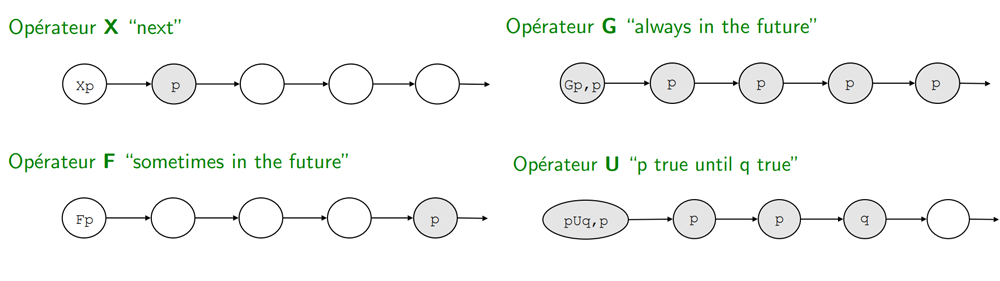
\includegraphics[scale=0.43]{figures/operateurs-temp.png}
   \caption[Caption for LOF]{Modalités temporelles de LTL \cite{bardin-slides}}
   \label{fig:operateurs-temp}
\end{figure} 

\subsubsection{Computation Tree Logic - CTL}
CTL est une logique temporelle basée sur la logique propositionnelle avec une notion discrète du temps dont le futur n'est pas déterminé. En effet, CTL exprime tous les chemins possibles d'un état à un autre grâce à sa structure d'arbre (notamment les arbres résultant du modèle de Kripke). En d'autres termes, la logique temporelle arborescente CTL peut être définie à partir d’un ensemble de variables propositionnelles AP, des connecteurs classiques de la logique propositionnelle tels que l'implication, la conjonction ou la disjonction, de quantificateurs de chemins (E ou A) et de connecteurs temporels (X,F,G,U). La syntaxe et sémantique de CTL fera l'objet des \autoref{sec:syntaxe-CTL} et \autoref{sec:sem-CTL}. \\

\subsection{Syntaxe de CTL} \label{sec:syntaxe-CTL}
Avant de décrire la syntaxe de CTL, la notion de \textit{chemin} dans un système de transition (en particulier, celle de Kripke ) est à définir : 

\noindent\fbox{\parbox{\linewidth\fboxrule\fboxsep}{Un \textbf{chemin} $\pi$ dans un système de Kripke $\mathcal{K} = (S,I,A,AP,\delta,\lambda)$ est une séquence infinie d'états $s_{0}, s_{1}, \dots \in S$ tel que $\forall i \ge 0 : s_{i} \rightarrow s_{i+1}$.}}  \\

Comme expliqué précédemment, la logique temporelle arborescente CTL est basée sur la logique propositionnelle et définit donc chaque connecteur de cette logique ainsi que d'autres connecteurs temporels propres à CTL. Cet ensemble forme la syntaxe de la logique temporelle arborescente CTL et est présentée comme tel : \\

Soit: \\
$\mathbb{V}$ un ensemble de variables propositionnelles, \\
$C$ un ensemble fini de connecteurs propositionnels: $C = \{\wedge, \vee, \neg, \Rightarrow, \Leftrightarrow \}$, \\
$T$ un ensemble fini de connecteurs temporels : $T = \{X, F, G, U, A, E\}$ \\

Tel que:\\
$\mathbb{V} \subseteq CTL$ (variables propositionnelles sont donc des formules CTL), \\
$\phi$, $\phi_{1}, \phi_{2}$ des propriétés quelconques $\in CTL$ \\

Alors: \\

\begin{center}
\begin{tabular}{|c|c|c|}
  \hline
  Syntaxe & Notation française & Signification \\
  \hline
  $\neg\phi_{1}$ & NON $\phi_{1}$ & Négation de $\phi_{1}$ \\
  $\phi_{1} \wedge \phi_{2}$ & $\phi_{1}$ ET $\phi_{2}$ & Conjonction de $\phi_{1}$ et $\phi_{2}$\\
  $\phi_{1} \vee \phi_{2}$ & $\phi_{1}$ OU $\phi_{2}$ & Disjonction de $\phi_{1}$ et $\phi_{2}$\\
  $\phi_{1} \Rightarrow \phi_{2}$ & $\phi_{1}$ IMPLIQUE $\phi_{2}$ & Implication de $\phi_{1}$ vers $\phi_{2}$\\
  $\phi_{1} \Leftrightarrow \phi_{2}$ & $\phi_{1}$ EQUIVAUT $\phi_{2}$ & Double implication (équivalence) de $\phi_{1}$ et $\phi_{2}$\\
 \hline
 
\end{tabular}
\captionof{table}{Syntaxe de CTL - Logique propositionnelle} \label{tab:syntax-ctl-prop}
\end{center}

\begin{center}
\begin{tabular}{|c|c|c|}
  \hline
  Syntaxe & Signification \\
  \hline
  $AX\phi$ & Dans tous les chemins ($A$), $\phi$ est satisfait pour le prochain état du chemin. ($X$)\\
  $AF\phi$ & Dans tous les chemins ($A$), $\phi$ est satisfait pour au moins un état du chemin. ($F$) \\
  $AG\phi$ & Dans tous les chemins ($A$), $\phi$ est satisfait pour tous les états du chemin. ($G$) \\
  $A(\phi_{1} \cup \phi_{2})$ & Dans tous les chemins ($A$), $\phi_{1}$ est satisfait jusqu'à ce que $\phi_{2}$ devient valide ($\cup$) \\
  \hline
  $EX\phi$ & Il existe un chemin ($E$) où $\phi$ est satisfait pour le prochain état du chemin. ($X$) \\
  $EF\phi$ & Il existe un chemin ($E$) où $\phi$ est satisfait pour au moins un état du chemin. ($F$)\\
  $EG\phi$ & Il existe un chemin ($E$) où $\phi$ est satisfait pour tous les états du chemin. ($G$)\\
  $E(\phi_{1} \cup \phi_{2})$ & Il existe un chemin ($E$) où $\phi_{1}$ est satisfait jusqu'à ce que $\phi_{2}$ devienne satisfait ($\cup$) \\
  
 \hline
 
\end{tabular}
\captionof{table}{Syntaxe de CTL - Logique temporelle} \label{tab:syntax-ctl-temp}
\end{center}

La \autoref{tab:syntax-ctl-prop} reprend les connecteurs principaux de la logique propositionnelle tandis que la \autoref{tab:syntax-ctl-temp} correspondant à de la logique temporelle. Cette dernière est divisée selon les quantificateurs de chemins en deux parties : 
\begin{itemize}
\item \textbf{A} pour "\textbf{A}ll" : la propriété est satisfaite sur tous les chemins possibles (= inévitable).
\item \textbf{E} pour "\textbf{E}xists" : la propriété est satisfaite sur au moins un chemin (= possible).
\end{itemize}

Chacune de ses parties possède 4 types de connecteurs : 
\begin{itemize}
\item \textbf{X} pour "ne\textbf{X}t" : la propriété doit être satisfaite pour le prochain état du chemin. 
\item \textbf{F} pour "\textbf{F}inally" : la propriété est satisfaite pour au moins un état du chemin.
\item \textbf{G} pour "\textbf{G}lobally" : la propriété est satisfaite pour tous les états du chemin.
\item $\pmb{\cup}$ pour "\textbf{U}ntil" : la propriété doit être satisfaite jusqu'à ce que la deuxième est "déclenchée" et devient donc satisfaite. \\
\end{itemize}

La logique temporelle présentée à la \autoref{tab:syntax-ctl-temp} est illustrée dans la \autoref{fig:syntax-schema}. Les propositions de l'état initial de chaque système sont considérés comme étant vraies. 

\begin{figure}
  \centering
   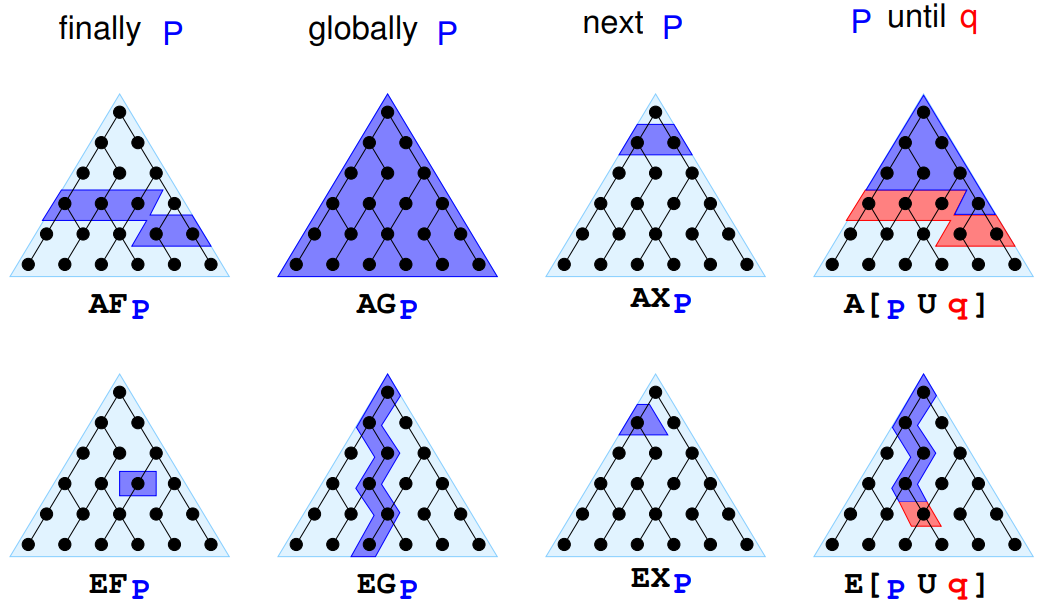
\includegraphics[scale=0.43]{figures/syntax-schema.png}
   \caption[Caption for LOF]{Illustration de la logique temporelle de CTL \cite{artale-slides}}
   \label{fig:syntax-schema}
\end{figure}

\subsection{Sémantique de CTL} \label{sec:sem-CTL}
%Présentation de la sémantique de CTL - des relations de satisfactions, des interprétations des différentes formules, etc.. 
Les formules CTL sont interprétées par rapport aux états et aux chemins d'un système de transition (qui suit la structure de Kripke\footnote{cfr. \autoref{sec:kripke}}). Généralement, la sémantique de CTL aborde donc une formule CTL (propriété) $\phi$ par deux relations de satisfactions, une pour les états $s$ et l'autre pour les chemins\footnote{Rappel: la notion de chemin est définie dans la \autoref{sec:syntaxe-CTL}} $\pi \in \mathbb{P}$, où $\mathbb{P}$ définit l'ensemble des chemins $\{\pi_{0}, \pi_{1}, \dots, \pi_{i}\}$ d'une structure de Kripke : 

\begin{enumerate}
\item Pour un état :  $(\mathcal{K},s) \vDash \phi \Leftrightarrow s$ satisfait $\phi$ 
\item Pour un chemin : $(\mathcal{K},\pi) \vDash \phi \Leftrightarrow \pi$ satisfait $\phi$ 
\end{enumerate}

où $\mathcal{K} = (S,I,A,AP,\delta,\lambda)$ est une structure de Kripke.\\

Ces relations de satisfactions sont notamment définies par la logique propositionnelle : 

\begin{center}
\begin{tabular}{lll}
   $(\mathcal{K},s) \vDash \neg\phi$ & \hspace{0.5cm} $\Leftrightarrow$ \hspace{0.5cm} & $\neg s \vDash \phi$  \\
   $(\mathcal{K},s) \vDash \phi_{1} \wedge \phi_{2} $ & \hspace{0.5cm} $\Leftrightarrow$ \hspace{0.5cm} & $(s \vDash \phi_{1}) \wedge (s \vDash \phi_{2})$ \\
   $(\mathcal{K},s) \vDash \phi_{1} \vee \phi_{2} $ & \hspace{0.5cm} $\Leftrightarrow$ \hspace{0.5cm} & $(s \vDash \phi_{1}) \vee (s \vDash \phi_{2})$ \\
   %$(\mathcal{K},s) \vDash \exists\phi$ & \hspace{0.5cm} $\Leftrightarrow$ \hspace{0.5cm} & $\pi \vDash \phi$ pour minimum un chemin $\pi \in$ Chemins(s) \\ 
   %$(\mathcal{K},s) \vDash \forall\phi$ & \hspace{0.5cm} $\Leftrightarrow$ \hspace{0.5cm} & $\pi \vDash \phi$ pour tous les chemins $\pi \in$ Chemins(s) \\ 
\end{tabular}
\end{center}

De plus, pour vérifier la satisfaction d'une propriété $\phi$ d'une structure de Kripke $\mathcal{K}$ , la logique temporelle caractérise également la sémantique :

 
\begin{center}
\begin{tabular}{lll}
   $(\mathcal{K},s) \vDash AX\phi$ & \hspace{0.5cm} $\Leftrightarrow$ \hspace{0.5cm} & $\forall \pi \in \mathbb{P}$ tel que $s_{1} \vDash \phi$  \\
   $(\mathcal{K},s) \vDash AF\phi$ & \hspace{0.5cm} $\Leftrightarrow$ \hspace{0.5cm} & $\forall \pi \exists i\ge 0$ tel que $\pi_{i} \vDash \phi$ avec $\pi_{i} \in \mathbb{P}$  \\
   $(\mathcal{K},s) \vDash AG\phi$ & \hspace{0.5cm} $\Leftrightarrow$ \hspace{0.5cm} & $\forall \pi \forall i\ge 0$ : $\pi_{i} \vDash \phi$  avec $\pi_{i} \in \mathbb{P}$ \\
   $(\mathcal{K},s) \vDash A(\phi_{1} \cup \phi_{2})$ & \hspace{0.5cm} $\Leftrightarrow$ \hspace{0.5cm} & $(\forall \pi \exists i\ge 0$ tel que $\pi_{i} \vDash \phi_{2}) \wedge (\forall j \in 0 \le j < i$ : $\pi_{j} \vDash \phi_{1})$ avec $\pi_{i,j} \in \mathbb{P}$\\
   $(\mathcal{K},s) \vDash EX\phi$ & \hspace{0.5cm} $\Leftrightarrow$ \hspace{0.5cm} & $\exists \pi \in \mathbb{P}$ tel que $s_{1} \vDash \phi$  \\
   $(\mathcal{K},s) \vDash EF\phi$ & \hspace{0.5cm} $\Leftrightarrow$ \hspace{0.5cm} & $\exists \pi$ tel que $\exists i \ge 0$ tel que $\pi_{i} \vDash \phi$ avec $\pi_{i} \in \mathbb{P}$ \\
   $(\mathcal{K},s) \vDash EG\phi$ & \hspace{0.5cm} $\Leftrightarrow$ \hspace{0.5cm} & $\exists \pi$ tel que $\forall i\ge 0$ : $\pi_{i} \vDash \phi$  avec $\pi_{i} \in \mathbb{P}$\\
   $(\mathcal{K},s) \vDash E(\phi_{1} \cup \phi_{2})$ & \hspace{0.5cm} $\Leftrightarrow$ \hspace{0.5cm} & $(\exists \pi$ tel que $\exists i \ge 0$ tel que $\pi_{i} \vDash \phi_{2}) \wedge (\forall j \in 0 \le j < i$ : $\pi_{j} \vDash \phi_{1})$ avec $\pi_{i,j} \in \mathbb{P}$\\
\end{tabular}
\end{center}

\subsubsection{Equivalence sémantique} 

Deux formules CTL $\phi_{1}$ et $\phi_{2}$ sont équivalents, dénoté $\phi_{1} \equiv \phi_{2}$, lorsqu'ils sont sémantiquements identiques, c'est-à-dire que pour chaque état $s$ : $s \vDash \phi_{1} \Leftrightarrow s \vDash \phi_{2}$.

\textbf{Exemples d'équivalence sémantique} \\ 

\begin{itemize}
\item Les lois de De Morgan formulés en CTL : \\

\begin{center}
$\neg AF\phi \equiv EG\neg\phi$ \\
$\neg EF\phi \equiv AG\neg\phi$ \\
$\neg AX\phi \equiv EX\neg\phi$ \\
\end{center}

\item Les lois d'expansions : \\

\begin{center}
$ AG\phi \equiv \phi \wedge AXAG\phi$ \\
$ EG\phi \equiv \phi \wedge EXEG\phi$ \\
$ AF\phi \equiv \phi \vee AXAF\phi$ \\
$ EF\phi \equiv \phi \vee EXEF\phi$ \\
$ A(\phi_{1}\cup\phi_{2}) \equiv \phi_{2} \vee (\phi_{1} \wedge AXA(\phi_{1}\cup\phi_{2})$ \\
$ E(\phi_{1}\cup\phi_{2}) \equiv \phi_{2} \vee (\phi_{1} \wedge EXE(\phi_{1}\cup\phi_{2})$ \\
\end{center}

\end{itemize}


\subsubsection{Sûreté et vivacité d'un système}

Deux définitions importantes concernant le bon fonctionnement d'un système peuvent maintenant être exprimées : 

\begin{enumerate}
\item Un système est dit \textbf{sûr} lorsqu'il est garanti que quelque chose de "mauvais" ne va jamais se produire et peut être exprimer par la formule CTL $AG\neg bad$.  Si ce n'est pas le cas alors il existe un nombre fini de contre-exemples. 
\item Un système est dit \textbf{vivant} lorsqu'il est garanti que quelque chose de "bon" va toujours se produire et peut être exprimer par la formule CTL $AGAFgood$. Si ce n'est pas le cas alors il existe un nombre fini de contre-exemples. 
\end{enumerate}



\subsection{Comparaison LTL/CTL}

\subsubsection{Caractéristiques générales}
\begin{itemize}
\item LTL est limité à une représentation linéaire du système mais ses connecteurs temporels permettent d'exprimer le futur ainsi que le passé notamment grâce à ses extensions de formules. Par exemple, l'opérateur $G$ "Always in the future" devient $G^{-1}$ "Always in the past". Chacun de ses opérateurs possède sa variante exprimant le passé. 
\item CTL offre une représentation complète en arbre présentant tous les chemins possibles et donc une grand nombre de propriétés potentiels exprimés, ce qui fait donc de lui un model-checking efficace. Néanmoins, les connecteurs temporels utilisés ne permettent d'exprimer uniquement le temps futur. 
\end{itemize} 


% A EXPLIQUER
\subsubsection{Expressivité}
\begin{itemize}
\item LTL décrit les propriétés d'une exécution à la fois. LTL est donc très expressif sur un chemin mais il n'y a aucune expressivité sur les futures possibles. 
\item CTL raisonne sur un comportement arborescent en considérant plusieurs exécutions possible en même temps. CTL pourrait donc manquer d'expressivité linéaire mais est très expressif concernant les futures potentiels. \\
\end{itemize}

De ce fait, certaines propriétés CTL (LTL) ne sont pas expressibles en LTL (CTL) ou est considéré d'une autre façon d'une logique à une autre. Pour citer des exemples : 

\begin{itemize}
 \renewcommand{\labelitemi}{\scriptsize$\bullet$}
 \item  $AGEF\phi$ (appelé \textit{"reset property"}) est une formule CTL qui n'est pas expressible en LTL.
 \item La formule CTL $AFAXp$ distingue les deux systèmes présentés dans la \autoref{fig:CTL-EXPR-2} tandis que la formule LTL $FXp$ ne le distingue pas. 
 
 \begin{figure}
  \centering
   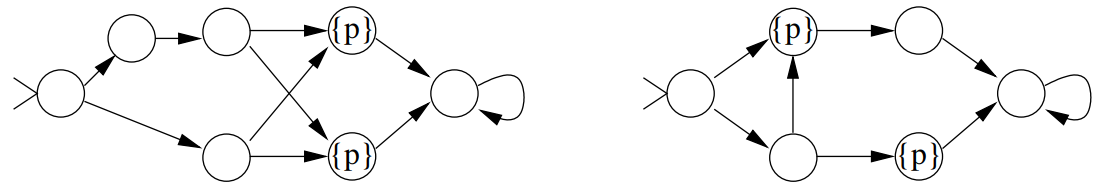
\includegraphics[scale=0.43]{figures/CTL-EXPR-2.png}
   \caption[Caption for LOF]{Exemple 2 - Expressivité CTL/LTL}
   \label{fig:CTL-EXPR-2}
\end{figure}

\item La formule LTL $FGp$ n'est pas expressible en CTL comme illustré dans la \autoref{fig:CTL-EXPR-3}. \\

 \begin{figure}
  \centering
   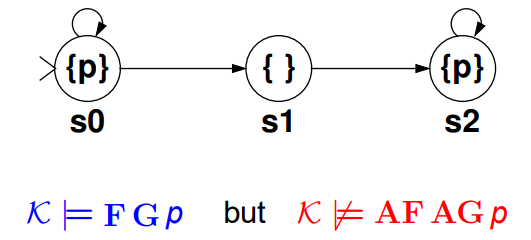
\includegraphics[scale=0.43]{figures/CTL-EXPR-3.png}
   \caption[Caption for LOF]{Exemple 3 - Expressivité CTL/LTL}
   \label{fig:CTL-EXPR-3}
\end{figure}

\end{itemize}

L'utilisation des deux types de logiques temporelles LTL et CTL est donc nécessaire ; l'expressivité de ces deux logiques n'est pas comparable, elles sont complémentaires : chaque logique possède des propriétés que l'autre ne peut pas exprimer. 

\subsubsection{Complexité théorique \\} 
\danger
\textit{Pour rappel, les notions de théorie de complexité abordés dans cette section sont présentées dans l'annexe \autoref{sec:complexity}.} 

\begin{itemize}
\item D'une part, la complexité en espace mémoire des problèmes de model checking utilisant LTL est PSPACE-complet. D'autre part, la complexité en temps de l'algorithme du model checking de LTL est en $\mathcal{O}(|TS| \cdot exp(|\phi|))$ où $|TS|$ correspond à la taille du système de transition et $|\phi|$ la taille de la propriété à vérifier. 
\item La complexité en temps des problèmes de model checking utilisant CTL est PTIME. Plus particulièrement, la complexité de l'algorithme du model checking de CTL est en $\mathcal{O}(|TS| \cdot |\phi|)$ où $|TS|$ correspond à la taille du système de transition et $|\phi|$ la taille de la propriété à vérifier. 
\end{itemize}


\subsubsection{En pratique}
\begin{itemize}
\item LTL (étendu avec des expressions régulières) est généralement utilisé dans l'industrie des processeurs. Il est notamment très intuitif au niveau des contres-exemples et de l'interface et permet la vérification au run-time par tests. LTL vérifie donc des propriétés compliquées mais uniquement sur des parties de système. 
\item CTL est utilisé pour une vérification de propriétés simples sur un système entier et donc en d'autres termes, effectue une vérification du modèle. 
\end{itemize}


\section{Le model-checking CTL: algorithme et implémentation}
\subsection{Présentation et analyse de l'algorithme}

L'algorithme de model checking de CTL qui va être présenté est le premier algorithme à avoir été développé, à savoir le model checking de CTL par labelling. 

\subsubsection{En quoi consiste l'algorithme par labelling ?} 

Premièrement, une structure de Kripke $\mathcal{K} = (S,I,A,AP,\delta,\lambda)$ ainsi qu'une certaine propriété $\phi$ à vérifier (formule CTL) sont prises en entrée. Comme son nom l'indique, l'algorithme par labelling se base sur des marquages tout au long de son exécution. Il est impossible de vérifier la propriété directement (sauf s'il s'agit d'une formule banale tels que $AF\phi$, $AX\phi$, ...), il est donc nécessaire de traiter les sous-formules $\phi '$ de $\phi$. Le marquage va donc s'opérer sur les états $s$ de $\mathcal{K}$ pour lesquels la sous-formule $\phi '$ est vérifiée. Cette opération de marquage est caractérisée par la fonction  \texttt{Marking($\mathcal{K}$,$\phi '$)} qui sera détaillée plus tard. S'en suit la même opération qui va être procédée récursivement pour les autres sous-formules. Finalement, $\mathcal{K}$ satisfait $\phi$ si et seulement si l'état initial $s_{0}$ est marqué par $\phi$.  

\subsubsection{Formules CTL à implémenter} 
Afin d'implémenter l'algorithme de model checking CTL par labelling, certaines formules CTL particulières sont à implémenter. Rappelons la liste des formules CTL\footnote{Rappel: cfr \autoref{sec:syntaxe-CTL} pour leurs significations} vues précédemment : 
$AX\phi$, $AF\phi$, $AG\phi$, $A(\phi_{1} \cup \phi_{2})$, $EX\phi$, $EF\phi$, $EG\phi$ et $E(\phi_{1} \cup \phi_{2})$ ainsi que les opérateurs de base en logique propositionnelle $\neg \phi$, $\phi_{1} \wedge \phi_{2}$ et $\phi_{1} \vee \phi_{2}$. Fort heureusement, uniquement les formules $EX\phi$, $E(\phi_{1} \cup \phi_{2})$ et $A(\phi_{1} \cup \phi_{2})$ sont essentielles à exprimer, du fait que les autres en découlent directement grâce aux relations d'équivalence.


\begin{center}
$ AX\phi \equiv \neg EX \neg \phi $ \\
$ AF\phi \equiv A(True \cup \phi) $ \\
$ AG\phi \equiv \neg EF \neg \phi $ \\
$ EF\phi \equiv E(True \cup \phi) $ \\
$ EG\phi \equiv \neg AF \neg \phi$ \\
\end{center}

Un algorithme de marquage pour les opérateurs de la logique propositionnelle ainsi que pour les trois formules CTL essentielles citées ci-dessus sera donc présenté dans les sections qui suivent. Les algorithmes présentées sont adaptés sur base du document de Sébastien Bardin : "Introduction au Model Checking", réalisé en 2008. \cite{Bardin-MC} \\  

\danger
\textbf{\textit{Remarque:}} Afin de clarifier les différents cas, la procédure de marquage a été divisée en différentes procédures mais il s'agit bien de la même fonction de marquage \texttt{Marking} qui regroupe les différents cas \texttt{MarkingNOT}, \texttt{MarkingAND}, \texttt{MarkingOR} ainsi que les autres procédures de marking concernant les formules CTL \texttt{MarkingEX}, \texttt{MarkingEU} et \texttt{MarkingAU}.

\subsubsection{Opérateurs de la logique propositionnelle} 

L'opération principale des différents algorithmes est évidemment le marquage des états qui vérifient la propriété $\phi$. Dans ce cas, $\phi = \neg \phi '$, $\phi = \phi_{1} \wedge \phi_{2}$ et $\phi = \phi_{1} \vee \phi_{2}$. Pour rappel, la procédure prend en input la structure de Kripke $\mathcal{K} = (S,I,A,AP,\delta,\lambda)$ et la formule à vérifier $\phi$. La notation $s.\phi$ fait le lien entre l'état $s$ et la formule $\phi$. Dans ce cas, l'état $s$ est étiquetté par le label $\phi$. En d'autres termes, si $s.\phi = True$ alors $s$ vérifie la formule $\phi$ et inversément.   

\begin{algorithm}
  \caption{Fonction de marquage : cas 1 $\phi = \neg\phi '$}\label{euclid}
  \begin{algorithmic}[1]
  \Procedure{MarkingNOT}{$\mathcal{K}$, $\phi$}
  \Comment{Cas 1: $\phi = \neg \phi '$}{}
  \State $\func{MarkingNOT}(\mathcal{K}, \phi ')$
  \Comment{Appel récursif de la fonction de marquage sur la sous-formule $\phi '$} 
  \ForAll{$\var{s}$ in $\var{S}$}:
  \State $s.\phi := not(s.\phi ')$
  \Comment{On redéfinit $s.\phi$ en l'assignant à la sous-formule $\neg\phi'$} 
  \EndFor
  \EndProcedure
  \end{algorithmic}
\end{algorithm}

\begin{algorithm}
  \caption{Fonction de marquage : cas 2 $\phi = \phi_{1} \wedge \phi_{2}$}\label{euclid}
  \begin{algorithmic}[1]
  \Procedure{MarkingAND}{$\mathcal{K}$, $\phi$}
  \Comment{Cas 2: $\phi = \phi_{1} \wedge \phi_{2}$}{}
  \State $\func{MarkingAND}(\mathcal{K}, \phi_{1})$;
  \Comment{Appel récursif de la fonction de marquage sur la sous-formule $\phi_{1}$}
  \State $\func{MarkingAND}(\mathcal{K}, \phi_{2})$;
  \Comment{Appel récursif de la fonction de marquage sur la sous-formule $\phi_{2}$}
  \ForAll{$\var{s}$ in $\var{S}$}:
  \State $s.\phi := and(s.\phi_{1}, s.\phi_{2})$
  \Comment{On redéfinit $s.\phi$ en l'assignant à la sous-formule $\phi_{1} \wedge \phi_{2}$} 
  \EndFor
  \EndProcedure
  \end{algorithmic}
\end{algorithm}

\begin{algorithm}
  \caption{Fonction de marquage : cas 3 $\phi = \phi_{1} \vee \phi_{2}$}\label{euclid}
  \begin{algorithmic}[1]
  \Procedure{MarkingOR}{$\mathcal{K}$, $\phi$}
  \Comment{Cas 3: $\phi = \phi_{1} \wedge \phi_{2}$}{}
  \State $\func{MarkingOR}(\mathcal{K}, \phi_{1})$;
  \Comment{Appel récursif de la fonction de marquage sur la sous-formule $\phi_{1}$}
  \State $\func{MarkingOR}(\mathcal{K}, \phi_{2})$;
  \Comment{Appel récursif de la fonction de marquage sur la sous-formule $\phi_{2}$}
  \ForAll{$\var{s}$ in $\var{S}$}:
  \State $s.\phi := or(s.\phi_{1}, s.\phi_{2})$
  \Comment{On redéfinit $s.\phi$ en l'assignant à la sous-formule $\phi_{1} \vee \phi_{2}$} 
  \EndFor
  \EndProcedure
  \end{algorithmic}
\end{algorithm}

\newpage
\subsubsection{$EX\phi$ : Exists Next}

Concernant la formule CTL $EX\phi$, l'état qui nous intéresse est l'état $s'$ suivant l'état $s$. Comme toutes les autres formules, l'appel récursif de la fonction de marquage avec la sous-formule est prise en entrée pour débuter. S'en suit deux boucles, l'une permettant d'initialiser tous les états comme étant des états qui ne vérifient pas la formule CTL $\phi$ et l'autre qui réalise l'opération permettant de constater si la sous-formule $EX\phi$ est vérifiée. Cette deuxième boucle va donc parcourir toutes les paires d'états $(s,s')$ en vérifiant si l'état $s'$ qui suit l'état $s$ vérifie la sous-formule $\phi '$. Si c'est le cas, alors l'état $s$ vérifie bien la formule CTL $EX\phi$. 
   
\begin{algorithm}
  \caption{Fonction de marquage : cas 4 $\phi = EX\phi '$}\label{euclid}
  \begin{algorithmic}[1]
  \Procedure{MarkingEX}{$\mathcal{K}$, $\phi$}
  \Comment{Cas 4: $\phi = EX\phi '$}{}
  \State $\func{MarkingEX}(\mathcal{K}, \phi ')$;
  \Comment{Appel récursif de la fonction de marquage sur la sous-formule $\phi '$}
  
  \ForAll{$\var{s}$ in $\var{S}$}:
  \Comment{Initialisation des états} 
  \State $s.\phi := false$
  \EndFor
  
  \ForAll{$\var{(s,s')} \in \rightarrow$}:
  \Comment{Parcours des paires d'états (s,s') où s' est l'état successeur de s} 
  \If {$s'.\phi '$ = true}:
  \Comment{Vérification que l'état successeur vérifie $\phi '$} 
  \State $s.\phi := true$
  \EndIf  
  \EndFor
  
  \EndProcedure
  \end{algorithmic}
\end{algorithm}

\subsubsection{$E(\phi_{1} \cup \phi_{2})$ : Exists $\phi_{1}$ Until $\phi_{2}$}

$E(\phi_{1} \cup \phi_{2})$ est une formule s'intéressant à deux états tout comme $EX\phi$ mais cette fois, il ne s'agit pas nécessairement de l'état suivant mais de tous les états futurs à l'état courant $s$. L'élément qui nous intéresse est l'état qui effectue un changement de sous-formule $\phi_{1}$ vers $\phi_{2}$. Pour ce faire, une liste \texttt{marked} retenant les des états qui ont été étiquettés $\phi_{2}$ ainsi que les états $\phi{1}$ dont un de ses états successeurs $s'$ est étiquetté $\phi_{2}$ est nécessaire. \\
De la même manière que les derniers algorithmes présentés, celui-ci est caractérisé par l'appel récursif de la fonction de marquage sur les sous-formule ainsi que d'une initialisation des états $s.\phi$ qui sont mis à \texttt{false} ainsi que de la liste \texttt{marked}. Le corps de l'algorithme est formé d'une première boucle parcourant tous les états $s$ afin de ne retenir que les états étiquettés par $\phi_{2}$. Une deuxième boucle réalise l'étiquetage de ces états à la formule CTL de base $\phi$. Finalement, une dernière boucle imbriquée à la seconde est effectuée afin d'étiquetter les états $s$ respectant la formule $\phi$, c'est-à-dire pour lesquels un des états successeurs $s'$ a été étiquetté $\phi$. 
   
\begin{algorithm}
  \caption{Fonction de marquage : cas 5 $\phi = E(\phi_{1} \cup \phi_{2})$}\label{euclid}
  \begin{algorithmic}[1]
  \Procedure{MarkingEU}{$\mathcal{K}$, $\phi$}
  \Comment{Cas 5: $\phi = \phi = E(\phi_{1} \cup \phi_{2})$}{}
  \State $\func{MarkingEU}(\mathcal{K}, \phi_{1})$;
  \Comment{Appel récursif de la fonction de marquage sur la sous-formule $\phi_{1}$}
  \State $\func{MarkingEU}(\mathcal{K}, \phi_{2})$;
  \Comment{Appel récursif de la fonction de marquage sur la sous-formule $\phi_{2}$}
  
  \State $marked := \{\}$
  
  \ForAll{$\var{s}$ in $\var{S}$}:
  \Comment{Initialisation des états} 
  \State $s.\phi := false$
  \State $s.seenBefore := false$ 
  \EndFor
  
  \ForAll{$\var{s'}$ in $\var{S}$}:
  \Comment{Récupération des états étiquettés par $\phi_{2}$}
  \If {$s'.\phi_{2}$ = true}:
  \Comment{Vérification que l'état vérifie $\phi_{2}$} 
  \State $marked$ += $s'$
  \EndIf  
  \EndFor
  
  
  \Do
  	\State chose $s' \in marked$ 
  	\State $marked$ -= $s'$ ;  $s'.\phi = true$ 
    \ForAll{$(s,s') \in \rightarrow$} 
    \Comment {On vérifie que l'état $s$ prédécesseur à $s'$ vérifient bien $\phi_{1}$} 
    \If {$s.seenBefore = false$} 
    \Comment {Si $s$ n'a pas encore été traité}
    \State $s.seenBefore = true$
    \If {$s.\phi_{1} = true$}
    \State $marked$ += $s$ 
    \Comment {ajouté à marked pour être etiquetté $s.\phi$}
    
     
    \EndIf
    \EndIf
    \EndFor
    
  \doWhile{$marked \neq \{\}$}
  
  \EndProcedure
  \end{algorithmic}
\end{algorithm}
  
\newpage 

\subsubsection{$A(\phi_{1} \cup \phi_{2})$ : Always $\phi_{1}$ Until $\phi_{2}$}

L'algorithme de $A(\phi_{1} \cup \phi_{2})$ ressemble vraisemblablement à celui de $A(\phi_{1} \cup \phi_{2})$. La seule différence est qu'il est indispensable que \textbf{tous} les états $s$ précédant un état $s'$ vérifiant $\phi_{2}$ soient vérifiés par $\phi_{1}$. Cette condition va se traduire par une variable \texttt{s.degree} qui correspond au degré (niveau) de l'état $s$. Un degré 0 équivaut à la racine et à l'état initial $s_{0}$. L'objectif est que tous les degrés précédant celui de $s'$ (donc jusqu'à l'état initial, degré 0) soient vérifiés par $\phi_{1}$. (cfr. ligne 16 dans Algorithm 6)

\begin{algorithm} 
  \caption{Fonction de marquage : cas 6 $\phi = A(\phi_{1} \cup \phi_{2})$}\label{euclid}
  \begin{algorithmic}[1]
  \Procedure{MarkingAU}{$\mathcal{K}$, $\phi$}
  \Comment{Cas 6: $\phi = A(\phi_{1} \cup \phi_{2})$}{}
  \State $\func{MarkingAU}(\mathcal{K}, \phi_{1})$;
  \Comment{Appel récursif de la fonction de marquage sur la sous-formule $\phi_{1}$}
  \State $\func{MarkingAU}(\mathcal{K}, \phi_{2})$;
  \Comment{Appel récursif de la fonction de marquage sur la sous-formule $\phi_{2}$}
  
  \State $marked := \{\}$
  
  \ForAll{$\var{s}$ in $\var{S}$}:
  \Comment{Initialisation des états} 
  \State $s.\phi := false$
  \State $s.degree := degree(s)$ 
  \EndFor
  
  \ForAll{$\var{s'}$ in $\var{S}$}:
  \Comment{Récupération des états étiquettés par $\phi_{2}$}
  \If {$s'.\phi_{2}$ = true}:
  \Comment{Vérification que l'état vérifie $\phi_{2}$} 
  \State $marked$ += $s'$
  \EndIf  
  \EndFor
  
  
  \Do
  	\State chose $s' \in marked$ 
  	\State $marked$ -= $s'$ ;  $s'.\phi = true$ 
    \ForAll{$(s,s') \in \rightarrow$} 
    \Comment {On vérifie que les états $s$ prédécesseurs à $s'$ vérifient bien $\phi_{1}$} 
    \State $s.degree$ -= 1; 
    \If {$(s.degree = 0)$ and $(s.\phi_{1} = true)$ and $(s.\phi = false)$}
    \Comment {Tous les préc. traités\dots\footnotemark}
    \State {$marked$ += $s$}
    \Comment {ajouté à marked pour être etiquetté $s.\phi$}
    

    \EndIf
    \EndFor
    
  \doWhile{$marked \neq \{\}$}
  
  \EndProcedure
  \end{algorithmic}
  
\end{algorithm}

\footnotetext{Si on a bien traité tous les états précédents l'état $s'$ et que l'état initial vérifie $\phi_{1}$}

\subsection{Résultats} 

Afin d'illustrer les algorithmes abordés, une exécution de chaque algorithme sur la structure de Kripke (modélisation) du problème de distributeur de boissons va être présentée. 

\danger
\textbf{\textit{Remarque:}} Pour rappel, \textbf{l'exécution des algorithmes présentés se font sur la structure de Kripke passée en entrée.} Uniquement par souci de visibilité, les actions des transitions entre les états ne sont pas annotés. De plus, l'annexe \autoref{sec:algo-arbres} présente ces algorithmes sur les 3 premiers niveaux du dépliage en arbre (degrés) de la structure de Kripke afin d'avoir un autre point de vue (plus lisible) de l'exécution. 

\subsubsection{$EX\phi$}

La formule CTL que la fonction prend en entrée est $\phi$ qui correspond donc à $\phi = EX\phi'$. $\phi '$ correspond ici à la propriété lorsque le distributeur est dans le mode "sélection de boissons" (alias $s$). A la fin de l'exécution, et donc de la seconde boucle (représenté en vert dans la \autoref{fig:algo-graph-EX}), nous obtenons les états accepteurs représentés par un état "doublement encadré" qui vérifient la propriété $\phi$, à savoir $\{s_{1} ,a_{1}\}$ qui précèdent un état dont $\phi ' = true$ ainsi que les transitions $X \xrightarrow{\text{action}} Y$ permettant la satisfaisabilité de $\phi$ sont mises en évidence où dans ce cas, $X$ est un état précédant $\phi '$ et $Y$ un état qui satisfait $\phi '$. 


\begin{figure}
  \centering
   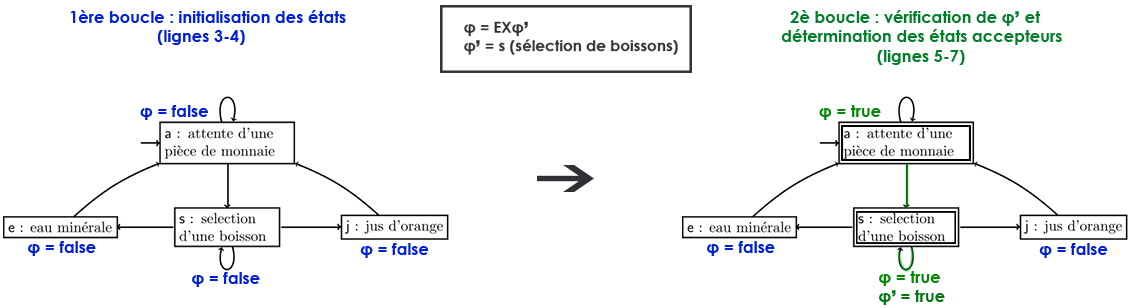
\includegraphics[scale=0.37]{figures/algo-graph-EX.png}
   \caption[Caption for LOF]{Exécution de l'algorithme 4 - $EX\phi$}
   \label{fig:algo-graph-EX}
\end{figure} 

\subsubsection{$E(\phi_{1} \cup \phi_{2})$}

La formule CTL que la fonction prend en entrée est $\phi$ qui correspond donc à $\phi = E(\phi_{1} \cup \phi_{2})$. $\phi_{1}$ correspond ici à la propriété lorsque le distributeur est en attente de la monnaie (alias $a$) et $\phi_{2}$ correspond au mode "sélection de boissons" (alias $s$). A la fin de la deuxième boucle (en bleu dans la \autoref{fig:algo-EU}), \texttt{marked} contient les états qui vérifient $\phi_{2}$, à savoir $\{s_{i}\}$ avec $0 \le i < \inf$. S'en suit la boucle principale (en vert dans la \autoref{fig:algo-graph-EU}) qui va vérifier les états prédécesseurs à \texttt{marked} = $\{s_{i}\}$. Les états $s_{i}$ vont être traités un par un et se voient retirés de \texttt{marked}. Les états satisfaisant $\phi_{1}$ vont être ajoutés à \texttt{marked} afin de passer leur étiquette $\phi$ à \texttt{true} pour finalement être retirés et obtenir une liste $marked$ vide qui marque la fin de la boucle. 


\begin{figure}
  \centering
   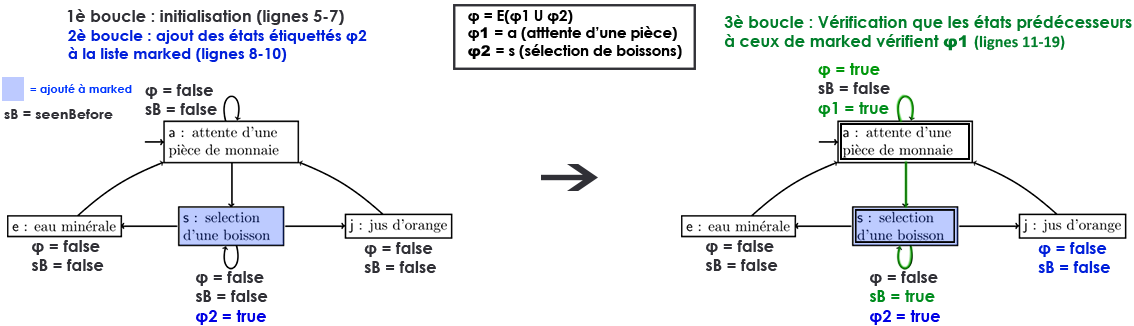
\includegraphics[scale=0.38]{figures/algo-graph-EU.png}
   \caption[Caption for LOF]{Exécution de l'algorithme 5 - $E(\phi_{1} \cup \phi_{2})$}
   \label{fig:algo-graph-EU}
\end{figure} 


\subsubsection{$A(\phi_{1} \cup \phi_{2})$}

La formule CTL que la fonction prend en entrée est $\phi$ qui correspond donc à $\phi = A(\phi_{1} \cup \phi_{2})$. $\phi_{1}$ et $\phi_{2}$ correspondent aux mêmes propriétés que précédemment pour $\phi = E(\phi_{1} \cup \phi_{2})$, à savoir respectivement $a$ et $s$. L'exécution est la même pour les 2 premières boucles sauf que dans ce cas-ci, nous avons besoin d'ajouter une variable \texttt{deg} (degré) à chaque état comme expliqué précédemment. Les variables de degré $d$ et $k$ correspondent au nombre de transitions $a_{i} \longrightarrow a_{i+1}$ et $s_{i} \longrightarrow s_{i+1}$. A la fin de la seconde boucle, \texttt{marked} contient donc toujours $\{s_{i}\}$. La boucle suivante (en vert dans la \autoref{fig:algo-AU}) tente de vérifier que tous les états prédécesseurs à ceux contenus dans \texttt{marked} vérifient $\phi_{1}$. Les états $a_{i}$ de la transition $a_{i} \xrightarrow{\text{insert\_coin()}} s_{i}$ ou de $a_{i} \longrightarrow a_{i+1}$ ne posent pas de soucis tandis que l'état prédecesseur $s_{j}$ de $s_{i}$ résultant de la transition $s_{j} \longrightarrow s_{i}$ (mis en évidence en rouge dans la \autoref{fig:algo-graph-AU}) ne satisfait pas $\phi_{1}$ qui engendre donc la non satisfaisabilité de la propriété $\phi$. 


\begin{figure}
  \centering
   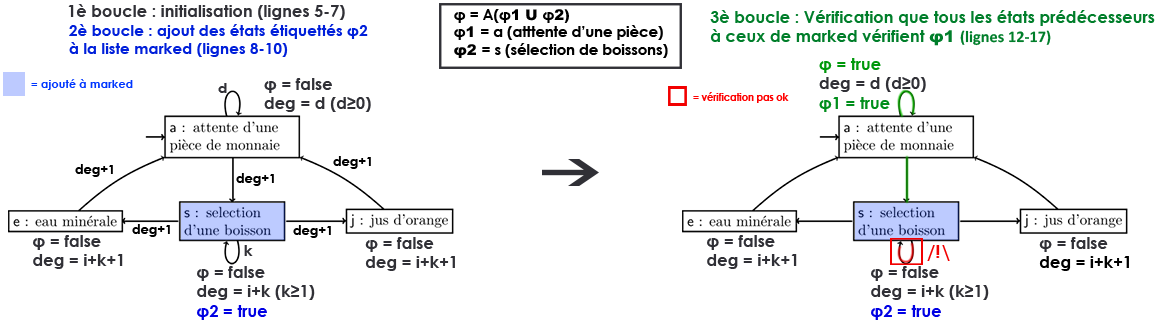
\includegraphics[scale=0.38]{figures/algo-graph-AU.png}
   \caption[Caption for LOF]{Exécution de l'algorithme 6 - $A(\phi_{1} \cup \phi_{2})$}
   \label{fig:algo-graph-AU}
\end{figure} 


\subsection{Complexité}

La complexité en temps des différents algorithmes présentés est caractérisée par des boucles parcourant la totalité des états du système, et serait donc en $\mathcal{O}(|TS|)$ avec $|TS|$ la taille du système. Néanmoins, comme cité précédemment, la complexité générale du model checking CTL ne se limite pas qu'à la taille du système mais dépends également de la taille de la formule CTL à vérifier. Dans notre cas, seules des formules basiques ont été traités, celles-ci prenant donc un temps de  $\mathcal{O}(1)$ mais dans des cas plus complexes, ce temps est évidemment à prendre en compte, ce qui nous amène à rappeler la complexité générale du model checking CTL qui est en $\mathcal{O}(|TS| \cdot |\phi|)$. \\


\section{Conclusion}

En conclusion, les bases de l'algorithme du model checking et plus particulièrement du model checking de CTL ont été vus. Le model checking CTL s'avère être une méthode de vérification automatique efficace, ceci se remarquant notamment à l'aide de l'algorithme par labelling présentée dans la section précédente. En effet, un avantage majeur de l'algorithme par labelling du model checking CTL est qu'il tourne en temps linéaire en chacune des entrées (structure de Kripke et formule CTL). L’algorithme repose sur le fait que toute formule CTL peut s’exprimer par un nombre restreint de formules sur les états. Cela nous permet de raisonner en termes d'états (satisfaisant la formule) plutôt que d’exécutions. \\

Néanmoins, nous avons vu que le model checking ne présente pas uniquement que des avantages et certains inconvénients tel que le \textit{state explosion problem} s'avèrent être impactant au niveau des performances du model checking. Malgré que certaines recherches aient déjà eu lieu, le model checking ne reste cependant pas parfait et peut donc faire objet de recherches supplémentaires quant à l'amélioration de celui-ci. 



\newpage
\begin{subappendices}
\renewcommand{\thesection}{\Alph{section}}%
% or try \arabic{section}

\section{Théorie de la complexité} \label{sec:complexity}

\subsection{Qu'est-ce que la théorie de la complexité ?}
La théorie de la complexité algorithmique s'intéresse à l'estimation de l'efficacité des
algorithmes et donc à l'étude formelle de la difficulté des problèmes en informatique. Deux types de complexité existent : 
\begin{itemize}
\item la complexité en \textbf{temps} : se base essentiellement sur le nombre d'opérations élémentaires (boucles, conditions, ...) pour traiter une donnée de taille $n$. 

\item la complexité en \textbf{espace mémoire} :  évalue l'espace mémoire utilisé en fonction de la taille des données.  
\end{itemize}

\subsection{Les machines de Turing déterministes et non déterministes}

\subsubsection{Machines de Turing déterministes} 
Les machines de Turing déterministes font toujours un seul calcul à la fois. Ce calcul est
constitué d'étapes élémentaires; à chacune de ces étapes, pour un état donné de la mémoire de la
machine, l'action élémentaire effectuée sera toujours la même.

\subsubsection{Machines de Turing non déterministes}
Une machine de Turing non déterministe est une variante théorique à une machine de Turing habituelle, qui, elle, est déterministe, mais s'en différencie dans le fait qu'étant non déterministe elle peut avoir plusieurs transitions activables, pour un état donné. À chaque étape de son calcul, cette machine peut donc effectuer un choix non-déterministe: elle a le choix entre plusieurs actions, et elle en effectue une. 

\subsection{Complexités PTIME \& PSPACE(-complet)}

\subsubsection{PTIME}
La classe P (ou PTIME) est la classe des problèmes de décision pour lesquels il existe un algorithme de résolution polynomial en temps (donc généralement rapide) par une
machine de Turing déterministe. Autrement dit, 

$$ PTIME = \bigcup_{k \in \mathbb{N}} TIME(n^{k}) $$

où $n$ est la taille de l'entrée et $TIME(t(n))$ est la classe des problèmes de décision qui peuvent être décidés en temps de l'ordre de grandeur de $t(n)$.

\subsubsection{PSPACE} 
PSPACE est la classe de complexité des problèmes de décision qui peuvent se résoudre sur une machine de Turing déterministe avec un espace polynomial. En d’autres termes, 

$$ PSPACE = \bigcup_{k \in \mathbb{N}} SPACE(n^{k}) $$

où $n$ est la taille de l'entrée et $SPACE(n^{k})$ est l'ensemble des problèmes de décision décidés par des machines de Turing déterministes utilisant un espace $t(n)$.

\subsubsection{PSPACE-complet}
Un problème $A$ est dit PSPACE-complet si les deux conditions suivantes sont remplies : 

\begin{itemize}
\item le problème $A$ est dans la classe PSPACE, c'est-à-dire $A \in PSPACE$,
\item tout problème PSPACE se réduit polynomialement à $A$, c'est-à-dire $\forall B \in PSPACE$ : $B \le_{p} A$. Si le problème $A$ vérifie cette condition, il est alors dit \textbf{PSPACE-dur}.
\end{itemize}

\newpage

\section{Exécution des algorithmes par labelling du MC CTL sur le dépliage en arbre de la structure de Kripke} \label{sec:algo-arbres}

\subsection{$EX\phi$}
\noindent
Etats accepteurs = $\{s_{1}, a_{1}\}$

\begin{figure}
  \centering
   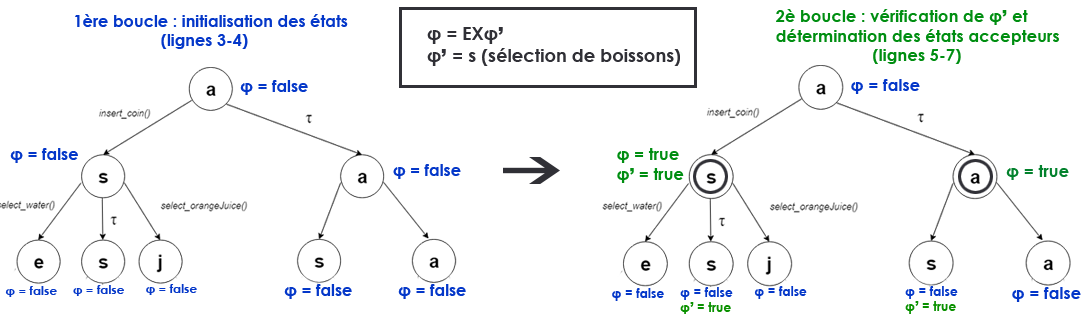
\includegraphics[scale=0.3]{figures/algo-EX.png}
   \caption[Caption for LOF]{Exécution de l'algorithme 4 - $EX\phi$}
   \label{fig:algo-EX}
\end{figure} 


\subsection{$E(\phi_{1} \cup \phi_{2})$}
\noindent
Etats accepteurs = $\{a_{0}, s_{1}, a_{1}, s_{2} '\}$ \\

\begin{figure}
  \centering
   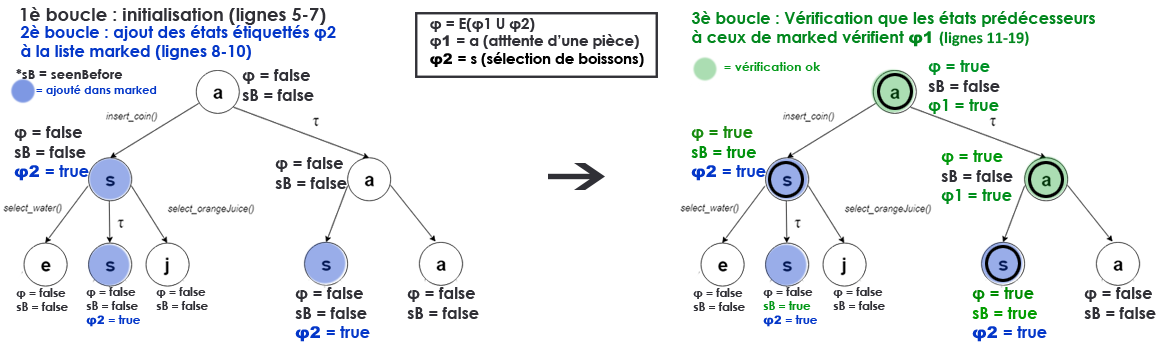
\includegraphics[scale=0.3]{figures/algo-EU.png}
   \caption[Caption for LOF]{Exécution de l'algorithme 5 - $E(\phi_{1} \cup \phi_{2})$}
   \label{fig:algo-EU}
\end{figure}

\subsection{$A(\phi_{1} \cup \phi_{2})$} 

\noindent
Etats accepteurs = $\{ \varnothing\}$ \\

\begin{figure}
  \centering
   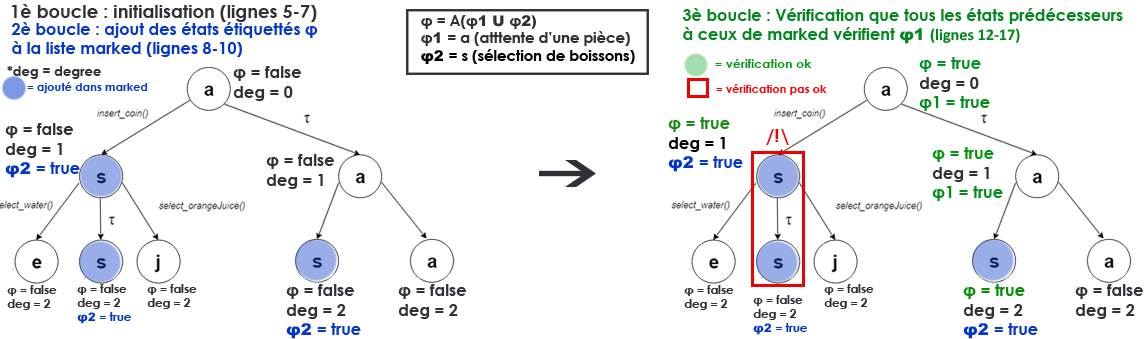
\includegraphics[scale=0.3]{figures/algo-AU.png}
   \caption[Caption for LOF]{Exécution de l'algorithme 6 - $A(\phi_{1} \cup \phi_{2})$}
   \label{fig:algo-AU}
\end{figure} 

\end{subappendices}

\bibliographystyle{unsrt}
\nocite{*}
\bibliography{bibliography}


\end{document}
